\documentclass[tikz,border=3pt]{standalone}
\usepackage{pgfplots}
\pgfplotsset{compat=1.17}
\definecolor{pdcsblue}{RGB}{0,114,178}
\definecolor{pdcsorange}{RGB}{213,94,0}
\begin{document}
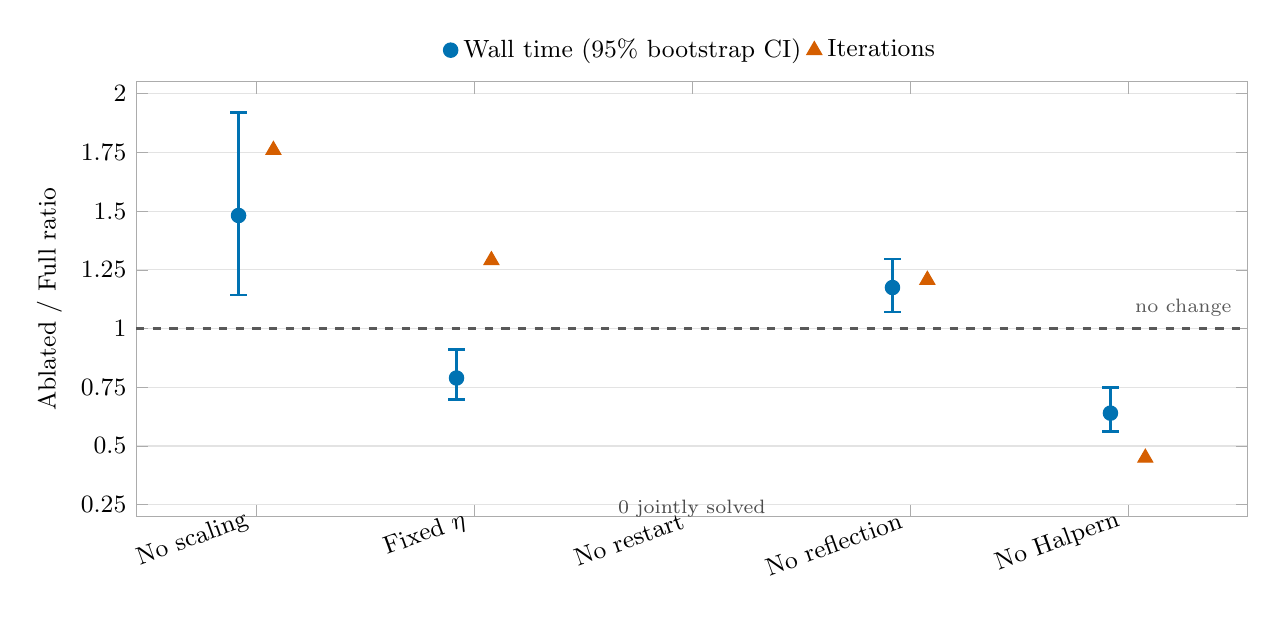
\begin{tikzpicture}
\begin{axis}[
  width=15.7cm,
  height=7.1cm,
  xmin=0.45,
  xmax=5.55,
  ymin=0.2,
  ymax=2.05,
  xtick={1,2,3,4,5},
  xticklabels={No scaling,Fixed $\eta$,No restart,No reflection,No Halpern},
  xticklabel style={rotate=20,anchor=east,font=\small},
  ytick={0.25,0.5,0.75,1,1.25,1.5,1.75,2},
  ylabel={Ablated / Full ratio},
  tick label style={font=\small},
  label style={font=\small},
  legend style={
    at={(0.5,1.02)},
    anchor=south,
    legend columns=2,
    draw=none,
    font=\small
  },
  ymajorgrids=true,
  grid style={gray!22},
  axis line style={gray!65},
  tick style={gray!65},
]
\addplot[black!65,dashed,line width=0.8pt,forget plot]
  coordinates {(0.45,1) (5.55,1)};
\node[anchor=south east,font=\scriptsize,text=black!65]
  at (axis cs:5.52,1.01) {no change};

\addplot+[
  only marks,
  mark=*,
  mark size=2.6pt,
  color=pdcsblue,
  mark options={fill=pdcsblue},
  error bars/.cd,
  y dir=both,
  y explicit,
  error bar style={line width=0.85pt},
  error mark options={rotate=90,mark size=3pt,line width=0.85pt},
] coordinates {
  (0.92,1.481153) += (0,0.43853345) -= (0,0.33961945)
  (1.92,0.78922451) += (0,0.12092087) -= (0,0.092124726)
  (3.92,1.1744282) += (0,0.12037819) -= (0,0.10414664)
  (4.92,0.63967685) += (0,0.10906446) -= (0,0.078898969)
};
\addlegendentry{Wall time (95\% bootstrap CI)}

\addplot+[
  only marks,
  mark=triangle*,
  mark size=3.1pt,
  color=pdcsorange,
  mark options={fill=pdcsorange},
] coordinates {
  (1.08,1.7596463)
  (2.08,1.290544)
  (4.08,1.2067563)
  (5.08,0.44944223)
};
\addlegendentry{Iterations}
\node[anchor=north,font=\scriptsize,text=black!70] at (axis cs:3,0.31) {0 jointly solved};
\end{axis}
\end{tikzpicture}
\end{document}
